\documentclass[10pt,a4paper]{article}
\usepackage[utf8]{inputenc}

% \usepackage{ngerman}  % german documents
\usepackage{graphicx}  % import graphics einbinden
\usepackage{listings}  % support source code listing
\usepackage{amsmath}  % math stuff
\usepackage{amssymb} % 
\usepackage{a4wide} % wide pages
\usepackage{fancyhdr} % nice headers
\usepackage{tikz} %graphs
\usetikzlibrary{arrows}
\lstset{basicstyle=\footnotesize,language=Python,numbers=left, numberstyle=\tiny, stepnumber=5,firstnumber=0, numbersep=5pt} % set up listings
\pagestyle{fancy}             % header
\setlength{\parindent}{0pt}   % no indentation

\usepackage[pdfpagemode=None, colorlinks=true,  % url coloring
           linkcolor=blue, urlcolor=blue, citecolor=blue, plainpages=false, 
           pdfpagelabels,unicode]{hyperref}
           
% change enums style: first level (a), (b), (c)           
\renewcommand{\labelenumi}{(\alph{enumi})}
\renewcommand{\labelenumii}{(\arabic{enumii})}

%lecture name
\newcommand{\lecture}{
	Bioinformatics III
}           

%assignment iteration
\newcommand{\assignment}{
	Fourth Assignment
}

%set up names, matricle number, and email
\newcommand{\authors}{
  \begin{tabular}{rl}
    \href{mailto:s9alfloh@stud.uni-saarland.de}{Alexander Flohr} & (2549738)\\
    \href{mailto:s9ankupi@stud.uni-saarland.de}{Andrea Kupitz} & (2550260)
  \end{tabular}
}

% use to start a new exercise
\newcommand{\exercise}[1]
{
  \stepcounter{subsection}
  \subsection*{Exercise \thesubsection: #1}

}

\begin{document}
\title{\Large \lecture \\ \textbf{\normalsize \assignment}}
\author{\authors}

\setlength \headheight{25pt}
\fancyhead[R]{\begin{tabular}{r}\lecture \\ \assignment \end{tabular}}
\fancyhead[L]{\authors}


\setcounter{section}{4} % modify for later sheets, i.e. 2, 3, ...
%\section{Introduction to Python and some Network Properties} % optional, note that section invocation sets the section counter + 1, so adapt the setcounter command
\maketitle

\exercise{Dijkstra's algorithm for finding shortest paths}
\begin{enumerate}
\item Figure \ref{fig1_1} shows an example of a graph with one edge with negative edge weight, where Dijkstra's algorithm fails to find minimal paths.\\
If we take node 1 as the source node, the algorithm will chose node 4 as the second node and thus never find the shortest path $1 \rightarrow 2 \rightarrow 4$ because nodes, that have been visited, are never visited again. Thereby, the algorithm returns the path $1 \rightarrow 4$ with length 2 as shortest path from 1 to 4 whereby the path $1 \rightarrow 2 \rightarrow 4$ with length -5 would be shorter.
\begin{figure}
\begin{center}
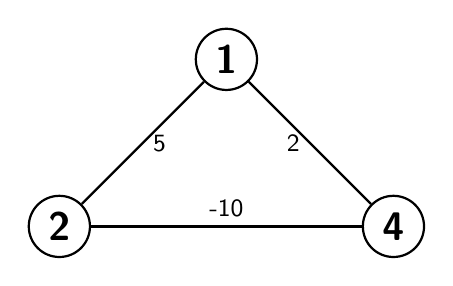
\begin{tikzpicture}[auto, node distance=3cm, every loop/.style={},
                    thick,main node/.style={circle,draw,font=\sffamily\Large\bfseries}]
  \label{fig1_1}
  \node[main node] (1) {1};
  \node[main node] (2) [below left of=1] {2};
  \node[main node] (4) [below right of=1] {4};
  \path[every node/.style={font=\sffamily\small}]
    (1) edge node [left] {2} (4)
    (2) edge node [right] {5} (1)
        edge node {-10} (4);
\end{tikzpicture}
\caption{example of network with negative edge weight}
\end{center}
\end{figure}

\item The modified algorithm guarantees to find the shortest path, even if some edges have negative weights because by adding the absolute value of the smallest edge weight to all weights, transforms the graph in a graph with only positive edge weights. In this way the original assumption holds that the total weight of a path can never get smaller than the weight of each edge in it. Formally, $\sum_{i \in path} w_i >= w_k \forall k \in path$

\item Breadth-first search can be applied in order to find shortest paths because it constructs a tree from the graph and visits all nodes. BFS is only guaranteed to find shortest paths if all edge weights are the same because the algorithm works with a queue and doesn't visit the nodes with minimal edge weights first like Dijkstra's algorithm. In this way BFS is only able to find path with minimal depth.
\end{enumerate}

\exercise{Force directed layout of networks}
\begin{enumerate}
\item Equation one and two show the force field for Coulomb energy, equation three and four for the harmonic energy.
\begin{equation}
\vec{F}_c(\vec{r}) = -\nabla E_c(\vec{r})
= -\frac{1}{4\pi\epsilon_0} \frac{q_1 q_2}{\nabla \|\vec{r}\|}
= -\frac{1}{4\pi\epsilon_0} \begin{pmatrix}
\frac{\delta}{\delta x} \frac{q_1 q_2}{\sqrt{x^2+y^2+z^2}} \\
\frac{\delta}{\delta y} \frac{q_1 q_2}{\sqrt{x^2+y^2+z^2}} \\
\frac{\delta}{\delta z} \frac{q_1 q_2}{\sqrt{x^2+y^2+z^2}} 
\end{pmatrix}
= -\frac{1}{4\pi\epsilon_0} \begin{pmatrix}
q_1 q_2 / \frac{x}{\sqrt{x^2+y^2+z^2}} \\
q_1 q_2 / \frac{y}{\sqrt{x^2+y^2+z^2}} \\
q_1 q_2 / \frac{z}{\sqrt{x^2+y^2+z^2}} 
\end{pmatrix}
\end{equation}
\begin{equation}
= -\frac{1}{4\pi\epsilon_0} \begin{pmatrix}
\frac{q_1 q_2 \sqrt{x^2+y^2+z^2}}{x} \\
\frac{q_1 q_2 \sqrt{x^2+y^2+z^2}}{y} \\
\frac{q_1 q_2 \sqrt{x^2+y^2+z^2}}{z} 
\end{pmatrix}
= -\frac{1}{4\pi\epsilon_0} q_1 q_2 \sqrt{x^2+y^2+z^2} \begin{pmatrix}
\frac{1}{x} \\
\frac{1}{y} \\
\frac{1}{z} 
\end{pmatrix}
= -\frac{1}{4\pi\epsilon_0} \frac{q_1 q_2 \|\vec{r}\|}{\vec{r}}
\end{equation}
\begin{equation}
\vec{F}_h(\vec{r}) = -\nabla E_h(\vec{r})
= -\frac{k}{2} \nabla \|\vec{r}\|^2
= -\frac{k}{2} \nabla (\sqrt{x^2+y^2+z^2})^2
= -\frac{k}{2} \nabla (x^2+y^2+z^2)
\end{equation}
\begin{equation}
= -\frac{k}{2} \begin{pmatrix}
2x+y^2+z^2 \\
x^2+2y+z^2 \\
x^2+y^2+2z
\end{pmatrix}
\end{equation}

\item Equation five shows the force field for Coulomb energy, equation six for the harmonic energy.
\begin{equation}
\vec{F}_c(\vec{r}_{ij}) = -\nabla E_c(\vec{r}_{ij})
= -\frac{k_i k_j}{\nabla \|\vec{r}_{ij}\|}
= -\frac{k_i k_j \|\vec{r}_{ij}\|}{\vec{r}_{ij}}
\end{equation}
\begin{equation}
\vec{F}_h(\vec{r}_{ij}) = -\nabla E_h(\vec{r}_{ij})
= -\frac{1}{2} \nabla \|\vec{r}_{ij}\|^2
= -\frac{1}{2} \begin{pmatrix}
2(x_i-x_j) + (y_i-y_j)^2 \\
(x_i-x_j)^2 + 2(y_i-y_j)
\end{pmatrix}
\end{equation}

\item If the degree of the nodes increases or decreases, the Coulomb energy decreases or increases, too because the Coulomb energy is proportional to the product of the node degrees.\\
Whereas the harmonic energy doesn't change if the degree of the nodes changes about the same amount because only the distance of them accounts to this energy.

\item 

\item Listing \ref{ex2-1} shows source code.
\lstinputlisting[label=ex2-1,caption={Listing of source code}] {layout.py}

\item Listing \ref{ex2-1} shows source code.\\


\item Listing \ref{ex2-2} shows source code.
\lstinputlisting[label=ex2-2,caption={Listing of source code}] {layout_main.py}
\end{enumerate}

\exercise{Graph Modular Decomposition}
Figure \ref{fig3_1} shows the modular decomposition of the set of protein complexes.
\begin{figure}
\begin{center}
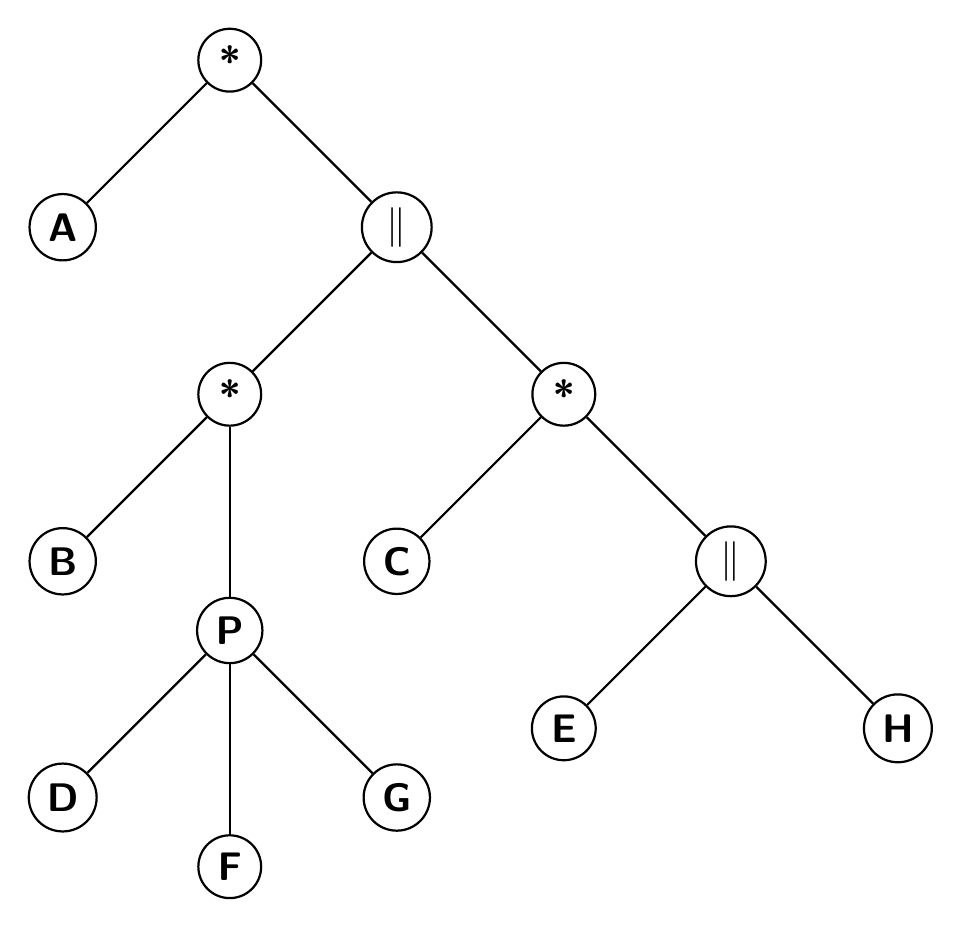
\begin{tikzpicture}[auto, node distance=3cm, every loop/.style={},
                    thick,main node/.style={circle,draw,font=\sffamily\Large\bfseries}]
  \label{fig3_1}
  \node[main node] (*1) {*};
  \node[main node] (A) [below left of=*1] {A};
  \node[main node] (1) [below right of=*1] {$\parallel$};
  \node[main node] (*2) [below left of=1] {*};
  \node[main node] (B) [below left of=*2] {B};
  \node[main node] (p) [below of=*2] {P};
  \node[main node] (*3) [below right of=1] {*};
  \node[main node] (D) [below left of=p] {D};
  \node[main node] (F) [below of=p] {F};
  \node[main node] (G) [below right of=p] {G};
  \node[main node] (C) [below left of=*3] {C};
  \node[main node] (2) [below right of=*3] {$\parallel$};
  \node[main node] (E) [below left of=2] {E};
  \node[main node] (H) [below right of=2] {H};
  \path[every node/.style={font=\sffamily\small}]
    (*1) edge node [left] {} (A)
    	edge node [right] {} (1)
    (1) edge node [left] {} (*2)
        edge node [right] {} (*3)
    (*2) edge node [left] {} (B)
         edge node [right] {} (p)
    (p) edge node [left] {} (D)
    	edge node {} (F)
        edge node [right] {} (G)
    (*3) edge node [right] {} (2)
    	 edge node [left] {} (C)
    (2) edge node [left] {} (E)
    (2) edge node [right] {} (H);
\end{tikzpicture}
\caption{modular decomposition of set of protein complexes}
\end{center}
\end{figure}

\end{document}